\documentclass{article}

\usepackage[english]{babel}
\usepackage{authblk}
\usepackage[a4paper,top=2cm,bottom=2cm,left=3cm,right=3cm,marginparwidth=1.75cm]{geometry}
\usepackage{amsmath}
\usepackage{graphicx}
\usepackage[colorlinks=true, allcolors=blue]{hyperref}
\usepackage{gensymb}
\usepackage{textcomp}

\title{Predicting Ensemble Width and Location in Binaural Recordings of Music with Convolutional Neural Networks}
\author[1]{Paweł Antoniuk*}
\author[1]{Sławomir Zieliński}
\affil[1]{Faculty of Computer Science, Białystok University of Technology, 15-351 Białystok, Poland; pawel.antoniuk@sd.pb.edu.pl}
\affil[*]{Corresponding author: pawel.antoniuk@sd.pb.edu.pl}

\date{}

\begin{document}
\maketitle

\begin{abstract}
Binaural audio technology has been around for many years, but its popularity has dramatically increased over the past decade due to advancements in virtual reality and streaming technologies. Along with its growing popularity, the quantity of publicly accessible binaural audio materials has also expanded. Consequently, there is now a need for automated and objective measurements of spatial content information, with ensemble width and location being the most important. In this study, 30 head-related transfer functions and 192 binaural music recordings from publicly accessible multi-track recording repositories were used to synthesize 23,040 binaural recordings. The synthesised recordings were then used to train a convolutional neural network prediction model, the aim of which was to predict the width and location of the ensemble for unseen recordings. The results indicate that models of ensemble breadth and position can be successfully constructed with low prediction errors --- $4.62\degree$ ($\pm0.09\degree$) degrees for ensemble location and $8.63\degree$ ($\pm0.29\degree$) degrees for ensemble width. This approach is the first of its kind to predict both ensemble width and location, offering a more accurate representation of spatial properties. This suggests significant potential for advancing spatial audio applications in virtual reality and streaming technologies, by providing audio engineers with tools that can leverage these methods to enhance spatial audio experiences.
\end{abstract}


\section{Introduction}
\section{Related studies}



\section{Methodology}

Experiments in this study were conducted on 2340 binaural recordings of music. The binaural recordings were synthesized semi-automatically using 192 multi-track publicly-available music recordings and 30 HRTF databases. For each multi-track recording and HRTF database pair, four binaural recordings were synthesized for different random ensemble parameters --- its location $\phi$ and width $\theta$ --- as defined in Section \ref{subsec:ensemble-definition}. Both parameters were drawn from uniform random distribution.

\subsection{Ensemble location and width definition}
\label{subsec:ensemble-definition}

The primary objective of the model developed in this study is to predict the ensemble location ($\theta$) and width ($\omega$), as illustrated in Figure \ref{fig:scene}. The ensemble is defined as a group of audio point sources. The ensemble width $\omega$ is defined as the angular width between two extreme point sources, while the ensemble location $\theta$ represents the middle angle between two extreme sound sources.

\begin{figure}
\centering
\includegraphics[width=\linewidth]{../pictures/scene.png}
\caption{\label{fig:scene}Illustration of ensemble width ($\omega$) and ensemble location ($\theta$) relative to the direction of the head. Black dots represent the positions of audio sources. The ensemble location ($\theta$) is defined as the angular position of the center of the ensemble relative to the direction the head is turned. The ensemble width ($\omega$) is defined as angular distance between two extreme audio sources. }
\end{figure}

\subsection{Synthesis of binaural music recordings}
\subsection{Spectrogram conversions of binaural music recordings}

\begin{figure}
\centering
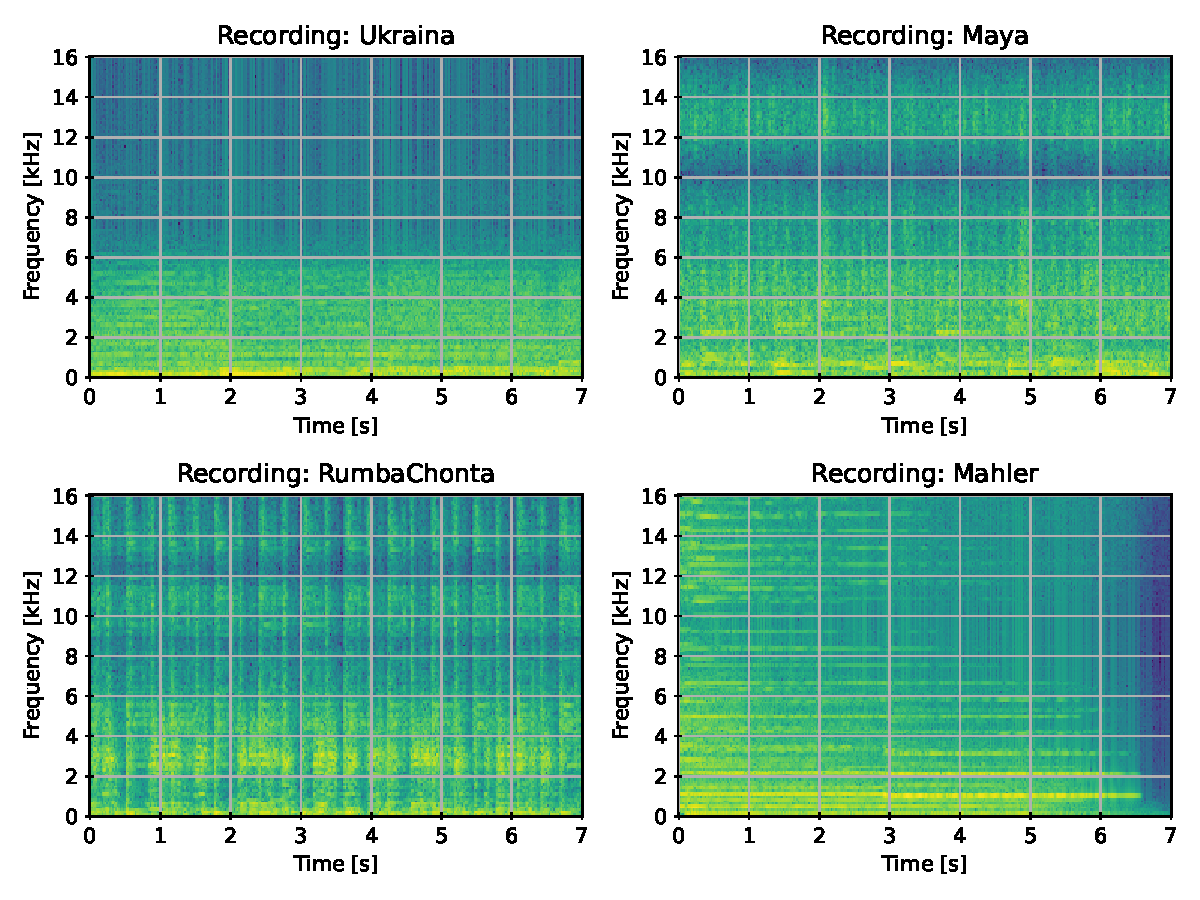
\includegraphics[width=\linewidth]{../figures/samples.pdf}
\caption{\label{fig:samples}An illustrative example of the magnitude spectrograms generated from synthesized binaural recordings of music. Each spectrogram was derived from a different randomly selected binaural music recording. These spectrograms were subsequently employed as input data for training and assessing the convolutional neural network (CNN) in this study. }
\end{figure}

Prior to being fed into the model, the binaural recordings of music were transformed into magnitude spectrograms. Figure \ref{fig:samples} illustrates example spectrograms for four distinct binaural recordings of music. It should be noted that the original spectrograms were stored in a floating-point-precision matrix format.

\subsection{Convolutional neural network topology}
\subsection{Model training and evaluation}
\section{Results}

\begin{figure}[ht]
  \centering
  \begin{minipage}[t]{0.45\linewidth}
    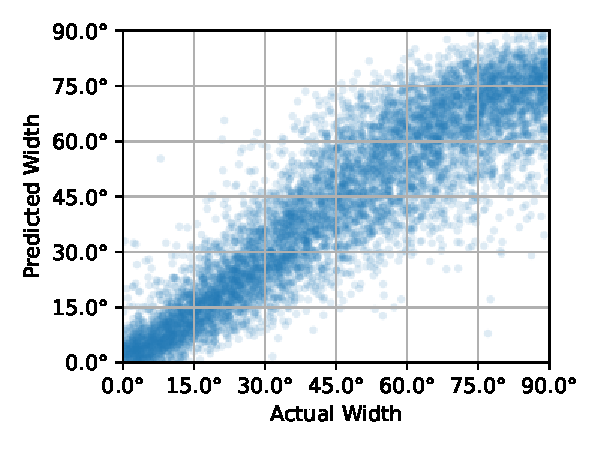
\includegraphics[width=\linewidth]{../figures/actual_vs_predicted_width.pdf}
    \caption{\label{fig:actual_vs_predicted_width}A comparison between the actual and the predicted ensemble width for a single iteration (of the total five) }
  \end{minipage}
  \hspace{0.5cm} 
  \begin{minipage}[t]{0.45\linewidth}
    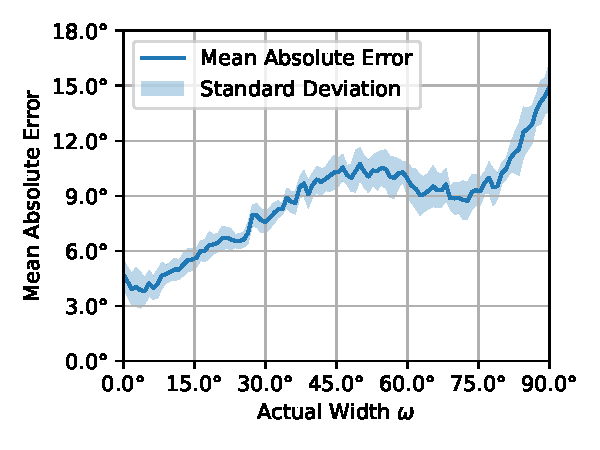
\includegraphics[width=\linewidth]{../figures/mae_width.pdf}
    \caption{\label{fig:mae_width}The impact of the actual ensemble width on the mean absolute prediction error, averaged across all five iterations, with indicated standard deviation.}
  \end{minipage}
\end{figure}

Figure \ref{fig:actual_vs_predicted_width} illustrates the comparison between the actual and the predicted ensemble width. The results demonstrate that the model exhibits optimal prediction quality for narrower ensemble widths ($X\degree$ for $Y\degree$) and that its performance deteriorates with the increase of the ensemble width ($Z\degree$ for $W\degree$). Figure \ref{fig:mae_width} further demonstrates that the relationship between the prediction error and the actual width is not linear, exhibiting a depression between 60 and 75 degrees. This suggests, that the ensemble width has a significant impact on the ensemble width estimation.

\begin{figure}[ht]
  \centering
  \begin{minipage}[t]{0.45\linewidth}
    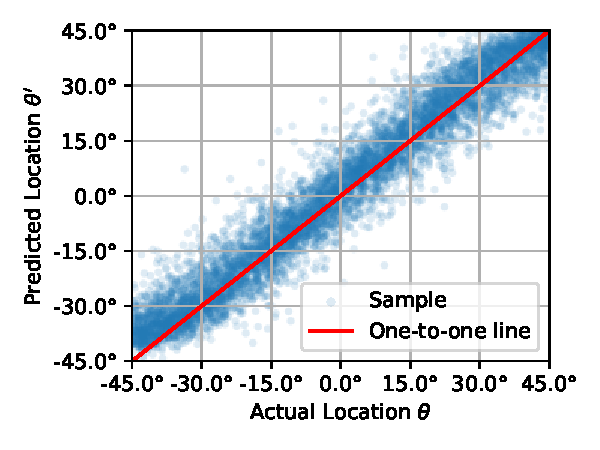
\includegraphics[width=\linewidth]{../figures/actual_vs_predicted_location.pdf}
    \caption{\label{fig:actual_vs_predicted_location}A comparison between the actual and the predicted ensemble location for a single iteration (of the total five) }
  \end{minipage}
  \hspace{0.5cm} 
  \begin{minipage}[t]{0.45\linewidth}
    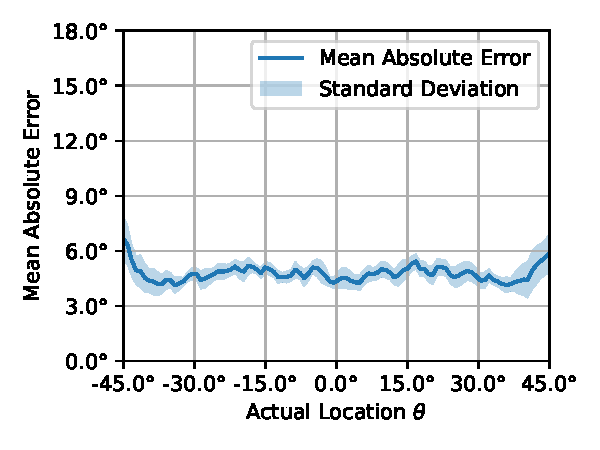
\includegraphics[width=\linewidth]{../figures/mae_location.pdf}
    \caption{\label{fig:mae_location}The impact of the actual ensemble width on the mean absolute prediction error, averaged across all five iterations, with indicated standard deviation.}
  \end{minipage}
\end{figure}

In contrast to the correlation between ensemble width and its prediction error, there is no significant relationship between the actual location and its prediction error, as illustrated in Figures \ref{fig:actual_vs_predicted_location} and \ref{fig:mae_location}. This finding indicates that the model's capabilities for localizing the center of the ensemble is robust, unaffected by the actual spatial positioning of the ensemble, including lateral locations.

\begin{figure}
    \centering
    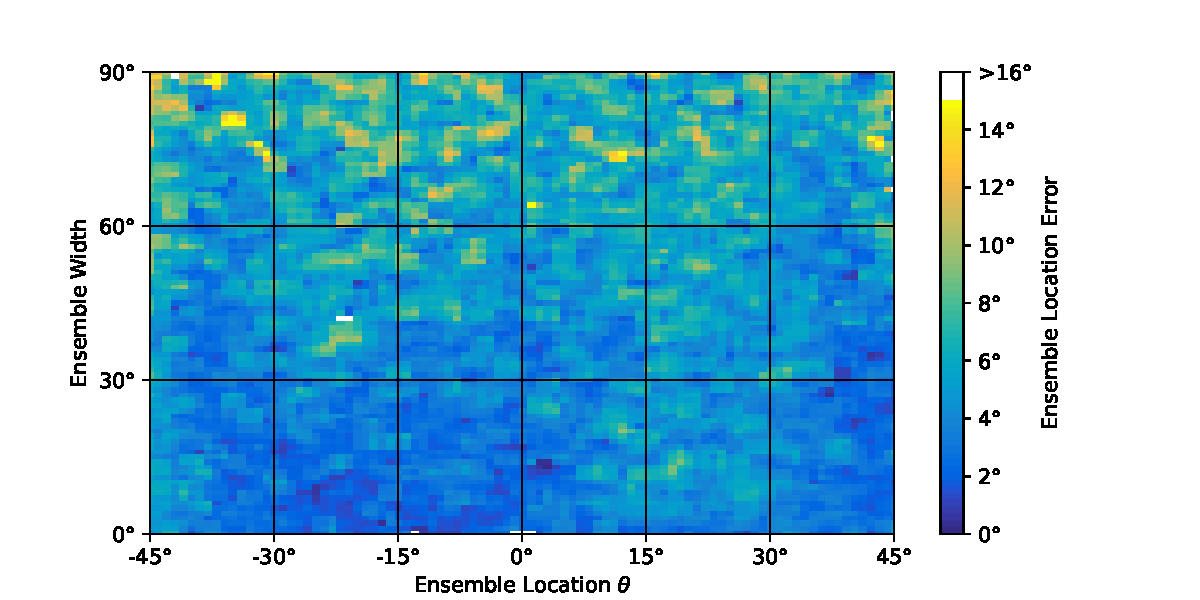
\includegraphics[width=\linewidth]{../figures/map_mae_location.pdf}
    \caption{\label{fig:map_mae_location}The heatmap that illustrates the mean absolute error (MAE) of ensemble location distribution across different ensemble locations (x-axis) and ensemble widths (y-axis). The color intensity corresponds to the MAE values, with lighter areas indicating higher errors.}
\end{figure}

Figure \ref{fig:map_mae_location} shows influence of both the ensemble width and location on mean absolute error for ensemble location. This shows more detailed view of data previously presented on Figure \ref{fig:mae_location}. The figure shows that there is a slight asymmetry. 

\begin{figure}
    \centering
    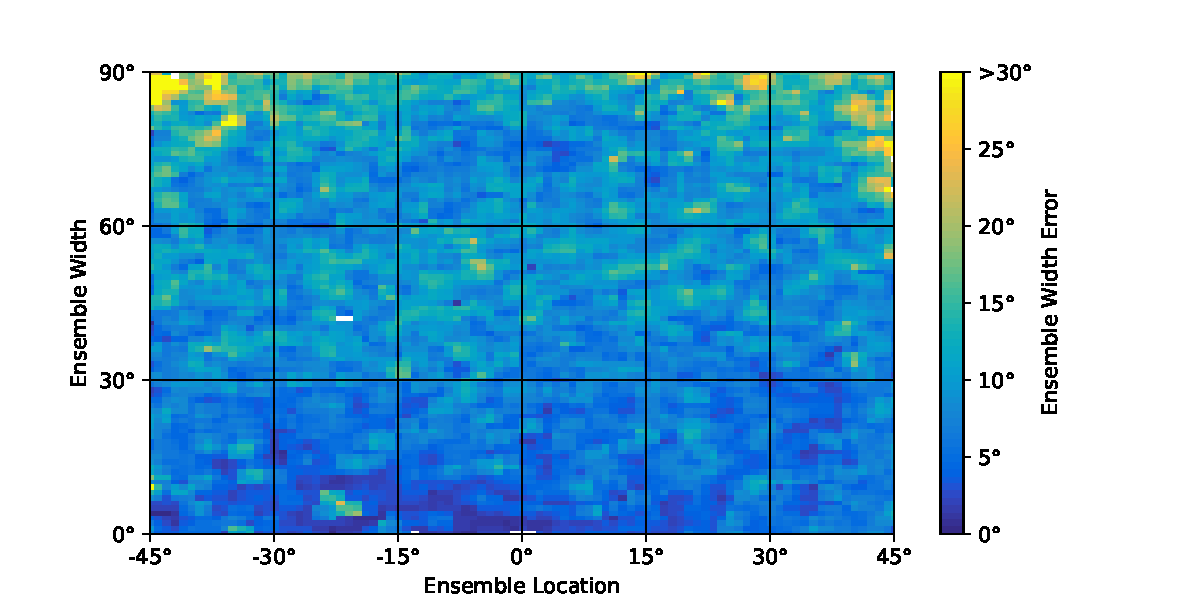
\includegraphics[width=\linewidth]{../figures/map_mae_width.pdf}
    \caption{\label{fig:map_mae_width}The heatmap that illustrates the mean absolute error (MAE) of ensemble width distribution across different ensemble locations (x-axis) and ensemble widths (y-axis). The color intensity corresponds to the MAE values, with lighter areas indicating higher errors. Notably, the values between $30\degree$ and $60\degree$ on the y-axis exhibit unexpectedly higher MAE values region --- please see Figure \ref{fig:mae_width} for comparison. }
\end{figure}

Similarly, Figure \ref{fig:map_mae_width} shows influence of both the ensemble width and location on mean absolute error for ensemble width.

\section{Conclusions}
\section{References}

\cite{greenwade93}

\bibliographystyle{alpha}
\bibliography{references}
\end{document}
